\documentclass[12pt]{amsart}
\pdfoutput=1
\usepackage{latexsym, amsmath, amssymb, amsthm, bm}
\usepackage{calrsfs}
\usepackage{subfig}

\usepackage[mathscr]{eucal}
\usepackage{mathtools}
\usepackage{paralist}
\usepackage[alphabetic]{amsrefs}
\usepackage[T1]{fontenc}
\usepackage{mathptmx}
\usepackage{microtype}
\usepackage{tikz}
\renewcommand{\baselinestretch}{1.05}
\usepackage[colorlinks=true,linkcolor=blue,urlcolor=blue, citecolor=blue]%
    {hyperref}
\linespread{1.06}
%%--LAYOUT--------------------------------------------------------------------
\usepackage[paperwidth=8.5in, paperheight=11in, inner=2.5cm, outer=2.5cm,% 
    top=2.5cm, bottom=2.5cm]{geometry}
%%--OTHER ENVIRONMENTS--------------------------------------------------------
\newtheorem{lemma}{Lemma}[section]
\newtheorem{theorem}[lemma]{Theorem}
\newtheorem{corollary}[lemma]{Corollary}
\newtheorem{proposition}[lemma]{Proposition}
\theoremstyle{definition}
\newtheorem{definition}[lemma]{Definition}
\newtheorem{remark}[lemma]{Remark}
\newtheorem{examplex}[lemma]{Example}
\newtheorem{procedure}[lemma]{Procedure}

\newenvironment{exm}
  {\pushQED{\qed}\renewcommand{\qedsymbol}{$\diamond$}\examplex}
  {\popQED\endexamplex}
\newtheorem{question}[lemma]{Question}
\newtheorem{conjecture}[lemma]{Conjecture}
\newtheorem{Construction}[lemma]{Construction}
\newtheorem{algorithm}[lemma]{Algorithm}
%\theoremstyle{remark}
\newcommand{\define}[1]{{\bfseries\itshape #1}}
%%--MATH----------------------------------------------------------------------
\newcommand{\relphantom}[1]{\mathrel{\phantom{#1}}}
\newcommand{\abs}[1]{\ensuremath{\left| #1 \right|}}
%\newcommand{\norm}[1]{\ensuremath{\left\| #1 \right\|}}
\newcommand{\ideal}[1]{\ensuremath{\left\langle #1 \right\rangle}}
\renewcommand{\geq}{\geqslant}
\renewcommand{\leq}{\leqslant}
\newcommand{\coloneq}{\ensuremath{\mathrel{\mathop :}=}}
\newcommand{\transpose}{\ensuremath{\textsf{\upshape T}}} 
%% Blackboard bolds symbols
\renewcommand{\AA}{\ensuremath{\mathbb{A}}} 
\newcommand{\CC}{\ensuremath{\mathbb{C}}} 
\newcommand{\kk}{\ensuremath{\Bbbk}} 
\newcommand{\NN}{\ensuremath{\mathbb{N}}}
\newcommand{\PP}{\ensuremath{\mathbb{P}}} 
\newcommand{\QQ}{\ensuremath{\mathbb{Q}}} 
\newcommand{\RR}{\ensuremath{\mathbb{R}}} 
\newcommand{\EE}{\ensuremath{\mathbb{E}}} 

\renewcommand{\P}{\ensuremath{P}} 
\newcommand{\Q}{\ensuremath{Q}} 

%\renewcommand{\SS}{\ensuremath{\mathbb{S}}} 
\newcommand{\ZZ}{\ensuremath{\mathbb{Z}}} 
%% Script symbols
\newcommand{\sC}{\ensuremath{\mathcal{C}}}
\newcommand{\sE}{\ensuremath{\mathcal{E}}}
\newcommand{\sF}{\ensuremath{\mathcal{F}}}
\newcommand{\calF}{\ensuremath{\mathcal{F}}}

\newcommand{\sH}{\ensuremath{\mathcal{H}}}
\newcommand{\sL}{\ensuremath{\mathcal{L}}}
\newcommand{\sO}{\ensuremath{\mathcal{O}}}
\newcommand{\diam}{\operatorname{diam}}
\newcommand{\Osh}{{\mathcal O}}
\newcommand{\Ish}{{\mathcal I}}
%% Operators
\DeclareMathOperator{\codim}{codim}
\DeclareMathOperator{\coker}{Coker}
\DeclareMathOperator{\conv}{conv}
\DeclareMathOperator{\Cox}{Cox}
\DeclareMathOperator{\depth}{depth}
\DeclareMathOperator{\gon}{gon}
\DeclareMathOperator{\Grass}{Gr}
\DeclareMathOperator{\green}{\textit{a}}
\DeclareMathOperator{\HH}{H}
\DeclareMathOperator{\HHH}{\mathbb{H}}
\DeclareMathOperator{\Hom}{Hom}
\DeclareMathOperator{\id}{id}
\DeclareMathOperator{\Image}{Im}
\DeclareMathOperator{\kept}{\lambda}
\DeclareMathOperator{\Ker}{Ker}
\DeclareMathOperator{\len}{\ell}
\DeclareMathOperator{\py}{py}
\DeclareMathOperator{\Pic}{Pic}
\DeclareMathOperator{\Proj}{Proj}
\DeclareMathOperator{\pr}{p}
\DeclareMathOperator{\qp}{qp}
\DeclareMathOperator{\qr}{qr}
\DeclareMathOperator{\rank}{rank}
\DeclareMathOperator{\reg}{reg}
\DeclareMathOperator{\Sos}{\Sigma}
\DeclareMathOperator{\Span}{Span}
\DeclareMathOperator{\Spec}{Spec}
\DeclareMathOperator{\sw}{sw}
\DeclareMathOperator{\Sym}{Sym}
\DeclareMathOperator{\topint}{int}
\DeclareMathOperator{\Tor}{Tor}
\DeclareMathOperator{\tw}{tw}
\DeclareMathOperator{\variety}{V}
%% Personalized comments
\newcommand\mv[1]{{\color{blue}(MV: #1)}}
\newcommand\mve[1]{{\color{red}(MV: #1)}}
\newcommand\jh[1]{{\color{red}(JH: #1)}}

\title{Notes on stopping times and the CD kernel}

\begin{document}
%\section{Computing exit time probabilities}



\subsection{Preliminaries and notations on reproducing kernels}

Let $Z$ be a compact topological space and let $\nu$ be a probability measure supported on $Z$. The set $C^0(Z,\RR)$ of continuous, real-vaued functions on $Z$ becomes a Hilbert space via the inner product $\langle f,g\rangle:=\EE_{\nu}\left(fg\right)=\langle fg,\nu\rangle$. If $V\subseteq C^0(Z,\RR)$ is a finite-dimensional vector space of functions then this space inherits a Hilbert space structure and in particular, for each $z\in Z$ there exists an element $\phi_z\in V^*=V$ which reproduces the evaluation at $z$ in the sense that the equality $\langle f,\phi_z\rangle = f(z)$ holds for every $f\in V$. Such operators define the kernel function $K: X\times X\rightarrow \RR$ via the formula $K(z,y):=\langle \phi_z,\phi_y\rangle$ which by construction satisfies the key {\it reproducing property}
\[\forall f\in V,\forall z\in Z\left(f(z)=\int_X K(z,y)f(y)d\nu(y)\right).\]
The kernel is completely determined by the measure $\nu$ and the subspace $V\subseteq C^0(Z,\RR)$ and when several measures and subspaces are involved we write $K_{\nu,V}(z,y)$ instead of $K(z,y)$ to make this dependence explicit.
The following two formulas are very useful for computing and understanding the basic properties of reproducing kernels:
\begin{enumerate}
\item If $p_1,\dots, p_m$ is any $\nu$-orthonormal basis for the subspace $V$ then
\[K_{\nu,V}(z,y)=\sum_{j=1}^m p_j(z)p_j(y)\] and furthermore
\item If $h_1,\dots, h_m$ is any basis for the subspace $V$ and $A_{ij}:=\EE_{\nu}\left(h_ih_j\right)$
then
\[K_{\nu,V}(z,y)=(h_1(z),\dots, h_m(z))A^{-1} (h_1(y),\dots, h_m(y))^t.\]
\end{enumerate}

Finally a key quantity associated to a kernel is the Christoffel function $\Lambda_{\nu,V}(z):=\frac{1}{K_{\nu,V}(z,z)}$, whose importance stems from the following variational characterization

\[\Lambda_{\nu,V}(z):=\inf_{f\in V}\frac{\int_Z f(y)^2d\nu(y)}{f^2(z)} =\inf_{f\in V}\left\{\int_Z f^2(y)d\nu(y):  f(z)=1 \right\}\]
which follows easily from the Cauchy-Schwartz inequality. 
If $Z\subseteq \RR^d$ and $V_n$ is the subspace defined as the restriction to $Z$ of polynomial functions of degree $\leq n$, the asymptotic behavior of the Christoffel function can often be used for density estimation, as shown in recent work of Lasserre, Pouwels and Putinar~\cite{LPP_article},\cite{LPPBook}. A concrete set-up where these estimations can be carried out are described in the following Theorem~\cite[Theorem 5.3.4]{LPPBook} of Lasserre, Pouwels and Putinar, which extends earlier work of Kroo and Lubistky~\cite{KrooLubitsky2013a}

\begin{theorem}\label{CD_Density_estimation} Assume $Z\subseteq\RR^d$ is a compact subset of $\RR^d$, $m(z)$ is a continuous function which is positive on $Z$, $\lambda$ is a Borel probability measure supported on $Z$ and $N(d)$ is a polynomial which satisfy the equality 
\[\lim_{n\rightarrow \infty} \sup_{z\in Z}\left(|N(n)\Lambda_{V_n,\lambda}(z)-m(z)|\right)=0.\]
If $\nu$ is a Borel-probability measure on $Z$ which is absolutely continuous with respect to $\lambda$ and having a continuous positive density $f:Z\rightarrow \RR_{+}$ then 
\[\lim_{n\rightarrow \infty} \sup_{z\in Z}\left(\left|N(n)\Lambda_{V_n,\mu}(z)-\frac{f(z)}{m(z)}\right|\right)=0.\]
\end{theorem}

\begin{examplex}\label{ex: unit_sphere}{\it The unit sphere in $\RR^d$.}
A basic examples for which the hypotheses of Theorem~\ref{CD_Density_estimation} holds is the sphere $S^{d-1}\subseteq \RR^d$ with its normalized area measure $\lambda$. In this case the invariance of the measure with respect to rotations implies that the function $K(z,z)$ is constant and the expression for $K(z,z)$ in terms of orthogonal polynomials allows us to compute that constant as the dimension of the space of polynomials restricted to the unit sphere. Since the sphere is defined by a single quadric, this dimension is given by the formula
\[N(n) := \binom{d+n}{n}-\binom{d+n-2}{n-2}\]
so $N(n)\Lambda_{V_n,\lambda}(z)-1=0$ for all $z\in Z$ and we can use $m(z)=1$ in the formula above to conclude that for any measure that is absolutely continuous with respect to $\lambda$ with a positive and continuous density $f(z)$ then this density can be estimated uniformly by
\[\lim_{n\rightarrow \infty} N(n)\Lambda_{V_n,\mu}(z)=f(z)\]
\end{examplex}


\begin{examplex}\label{ex: unit_ball} {\it The unit ball in $\RR^d$.} A similar result to Theorem~\ref{CD_Density_estimation} is available for the unit ball $B^{d}\subseteq \RR^d$. It is known (see~\cite[Lemma 4.2.1, Theorem 4.2.2]{LPPBook} and ~\cite[Theorem 1.3]{KrooLubitsky2013a}) that if $N(n):=\binom{n+d}{d}$ and $\lambda$ is the measure on the unit ball with Lebesgue density $m(x):=\frac{2}{\omega_d\sqrt{1+\|x\|_2^2}}$ where $\omega_d$ is the surface area of $S^{d-1}\subseteq \RR^d$ then for $x\in B^d$ we have
\[\lim_{n\rightarrow \infty} N(n)\Lambda_{\lambda, V_n}=
\begin{cases}
1\text{, if $\|x\|<1$}\\
\frac{1}{2} \text{, if $x=1$.}
\end{cases}
\]
as a result, for any regular measure $\mu$ on $B^d$ having positive and continuous density $h$ with respect to the Lebesgue measure on the ball, the equality $\lim_{n\rightarrow\infty}N(n)\Lambda_{\mu, V_n} = \frac{h(x)}{m(x)}= \frac{\omega_d}{2}h(x)\sqrt{1+\|x\|_2^2}$ holds uniformly on compact subsets of the interior of $B$.

\end{examplex}

\section{Computing occupation and exit location densities}

The method of moments allows us to obtain estimates of the moments of our occupation and exit location measures, together with error bars on those estimates. For many applications however, it would be more useful to know the {\it density} of the occupation measures and of the exit location measures (with respect to some natural measures on $\chi$ and $\partial \chi$ respectively). In this Section we outline a method, based on Christoffel-Darboux kernels, which allows us to construct sequences of functions converging to such densities. 
For simplicity we will state the Theorem for the unit ball in $\RR^n$ but the same method can be applied more generally as discussed in Remark~\ref{Rmk: Extensions} below. Throughout the section we let $V_n:=\RR[x_1,\dots, x_d]_{\leq n}$ and let $W_n$ be the restriction of the elements of $V_n$ to the unit sphere $S^{d-1}\subseteq \RR^d$. To estimate the occupation density on the unit ball and the exit location density on its boundary we propose the following procedure,


\begin{procedure}\label{algo} Given a diffusion with generator $\mathcal{L}$ and initial location $X(0)=\zeta$, a total degree $d>0$, an approximation degree $r>0$ and an integer offset $s>0$, carry out the following steps:


\begin{enumerate}
\item Fix a basis $\ell_1,\dots, \ell_{N}$ for $W_n$. For each pair of elements $\ell_i,\ell_j$ solve the problems $d_r^{\min}$ and $d_r^{\max}$ with $g:=\ell_i\ell_j$ and define our estimate $\hat{A}_{ij}$ for $\EE_{\nu}[\ell_i\ell_j]=\langle \ell_i\ell_j,\nu\rangle$ as their average.
\item Fix a basis $h_1,\dots, h_M$ for $V_{n-s}$. For each pair of elements $h_i,h_j$ of the basis find a polynomial $p_{ij}$ which solves the equation $\mathcal{L}(p_{ij})=h_ih_j$ and compute our estimate $\hat{B}_{ij}$ for $\EE_{\mu}[h_ih_j]=\langle h_ih_j,\mu\rangle$ via the formula
\[\langle h_ih_j,\mu\rangle = \widehat{\langle p_{ij},\nu\rangle} + p_{ij}(\zeta)\] 
where $\widehat{\langle p_{ij},\nu\rangle}$ is the average between the optimal values of problems $d_r^{\min}$ and $d_r^{\max}$ with $g:=p_{ij}$.
\item Define our CD-estimates for the exit location density on the unit sphere $\hat{f}(x)$ and the occupation density $\hat{h}$ on the unit ball respectively, by the formulas
\[\widehat{f(z)} := N(n)\widehat{\Lambda_{V_n,\nu}(z)}= \frac{N(n)}{v^t(z) \hat{A}^{-1}v(z)}\]
where $N(n)$ is defined in Example~\ref{ex: unit_sphere}, and
\[\widehat{h(x)} = N(n)\widehat{\Lambda_{V_n,\mu}(z)} = \frac{N(n)m(x)}{h^t(x)\hat{B}^{-1}h(x)}\]
where $m(x)$ and $N(n)$ are defined in Example~\ref{ex: unit_ball}.
\end{enumerate}
\end{procedure}

\begin{theorem}\label{Thm: CD-densities-estimation} If the following conditions hold
\begin{enumerate}
\item The exit location density is absolutely continuous and has a positive and continuous density with respect to the Lebesgue measure on the unit sphere $S^{d-1}$ and
\item The occupation density is absolutely continuous and has a positive and continuous density with respect to the equilibrium measure on the unit ball
\item There exists a sequence $s(n)$ of positive integers with $n-s(n)\rightarrow \infty$ such that for all sufficiently large $n$ the inclusion $\mathcal{L}(V_n)\supseteq V_{n-s(n)}$ holds.
\item The chosen approximation degrees $r(n)$ grow sufficiently quickly so as to guarantee 
\[\lim_{n\rightarrow \infty}\sup_{g\in V_n}|d_{r(n)}^{\max}(g)-d_{r(n)}^{\min}(g)|\rightarrow 0\]  
\end{enumerate}
then the estimates $\widehat{f}(z)$ and $\widehat{h}(x)$ defined in Procedure~\ref{algo} converge uniformly to the true exit location and occupation densities respectively as $n\rightarrow \infty$.
\end{theorem}
\begin{proof} If $\mu,\nu$ denote the occupation measure and the exit location measure respectively and $X(0)=\zeta$ then the Kolmogorov equation implies that for any twice-differentiable function $f$ we have 
\[\langle f,\nu\rangle + \langle \mathcal{L}f,\mu\rangle = f(\zeta)\]
If $\mathcal{L}(V_n)\supseteq V_{n-s(n)}$ then this process allows us to compute the polynomial moments of the occupation measure. Because if $h\in V_{n-s(n)}$ then there exists $p\in V_n$, which can be easily computed with linear algebra, with $\mathcal{L}p=h$. As a result 
\[\langle h,\mu\rangle = f(\zeta)-\langle p,\nu\rangle\]
so estimates of the exit location moments can be used to obtain estimates for the occupation moments. Such computations which can become as good as we want by increasing the approximation degree $r(n)$, allowing us to estimate the corresponding Christoffel functions as accurately as we wish.The theorem now follows from Theorems~\ref{CD_Density_estimation} and~\cite[Theorem 1.3]{KrooLubitsky2013a}.
\end{proof}

\begin{remark}\label{Rmk: Extensions} Procedure~\ref{algo} can be carried out to estimate occupation densities for sets whose {\it Equilibrium measure} is well understood, generalizing the density $m(x)$ from Example~\ref{ex: unit_ball}. See~\cite[Section 4.2]{LPPBook} for several such instances. Similarly, the assumption of Theorem~\ref{CD_Density_estimation} holds for several geometries beside spheres, see~\cite[pag.71]{LPPBook} for several interesting instances.
\end{remark}


\subsection{Computational examples}
In this section we illustrate the usefulness of Procedure~\ref{algo} for estimating occupation densities in the unit ball and exit location densities on the unit sphere for some diffusions. The code used for the results in this Section is available on github by clicking \href{https://github.com/mauricio-velasco/Exit_location_density_estimation.git}{[here]}.

\begin{examplex} {\it Brownian motion in the unit disc.} For the two-dimensional brownian motion in the unit disc we have $\mathcal{L}f=-\Delta(f)$. We wish to estimate the exit location and occupation densities with the methods of the previous section. 

In order to compute the moments $\EE_{\nu}[g]$ of the exit location measure of Brownian motion starting at an arbitrary point $\zeta_0 = (r_0,\theta_0)$ of the unit disc $D\subseteq \RR^2$ analytically, it suffices to find any harmonic function $u$ on the disc with $u=g$ on the boundary circle and to evaluate it at the point $x_0$. Recalling that the real and imaginary parts of any holomorphic function are harmonic we can easily obtain plenty of candidates, for instance for any integer $k$ the complex monomial $w^k$ gives raise to $r^k\cos(kz)$ and $r^k\sin(kz)$ and combining such functions we are able to compute the moments of all products of the natural fourier basis as summarized in the following table\\

\begin{center}
\begin{tabular}{c|c}
Product & Expected value at exit time\\
\hline
$\cos(kz)\cos(jz)$ & $\frac{r_0^{k+j}\cos((k+j)z)-r_0^{|k-j|}\cos((k-j)z)}{2}$\\
$\cos(kz)\cos(jz)$ & $\frac{r_0^{k+j}\cos((k+j)z)-r_0^{|k-j|}\cos((k-j)z)}{2}$\\
$\cos(kz)\cos(jz)$ & $\frac{r_0^{k+j}\cos((k+j)z)-r_0^{|k-j|}\cos((k-j)z)}{2}$\\
\end{tabular} 
\end{center}

Knowing the exact values of the moments we can compute the Resulting normalized Christoffel functions $\Lambda^{\nu}_d(z):=\frac{2d-1}{\vec{m}^t M^{-1}\vec{m}}$
where $\vec{m}$ is the vector of $2d+1$ components containing the fourier basis elements of order at most $d$ and $M$ is the matrix of moments of their products. The resulting exit location densities are shown in Figure~\ref{fig: exit_loc_densities} for various initial conditions. Note that the density becomes sharper near the center as the initial point of our browian motion is closer to the boundary and that the density estimates are very accurate even of we only know moments of rather low degree (only degrees $3,5,10,15,20$ are shown).


\begin{figure}
    \centering
    \subfloat[]{\includegraphics[width=0.30\textwidth]{CD_exit_Location_0.png}} 
    \subfloat[]{\includegraphics[width=0.30\textwidth]{CD_exit_Location_1.png}} 
    \subfloat[]{\includegraphics[width=0.30\textwidth]{CD_exit_Location_2.png}} 
    \caption{(A) $(r_0,\theta_0)=(0.25,0.0)$ (B) $(r_0,\theta_0)=(0.5,0.0)$ (C) $(r_0,\theta_0)=(0.75,0.0)$}
    \label{fig: exit_loc_densities}
\end{figure}

Alternatively, we can do similar calculations via SOS optimization, obtaining Figure~\ref{fig: exit_loc_densities_SOS}. We also apply the results in the previous Section to estimate the occupation density obtaining Figure~\ref{fig: Brownian_Occupation} on the ball.

\begin{figure}
    \centering
    \subfloat[]{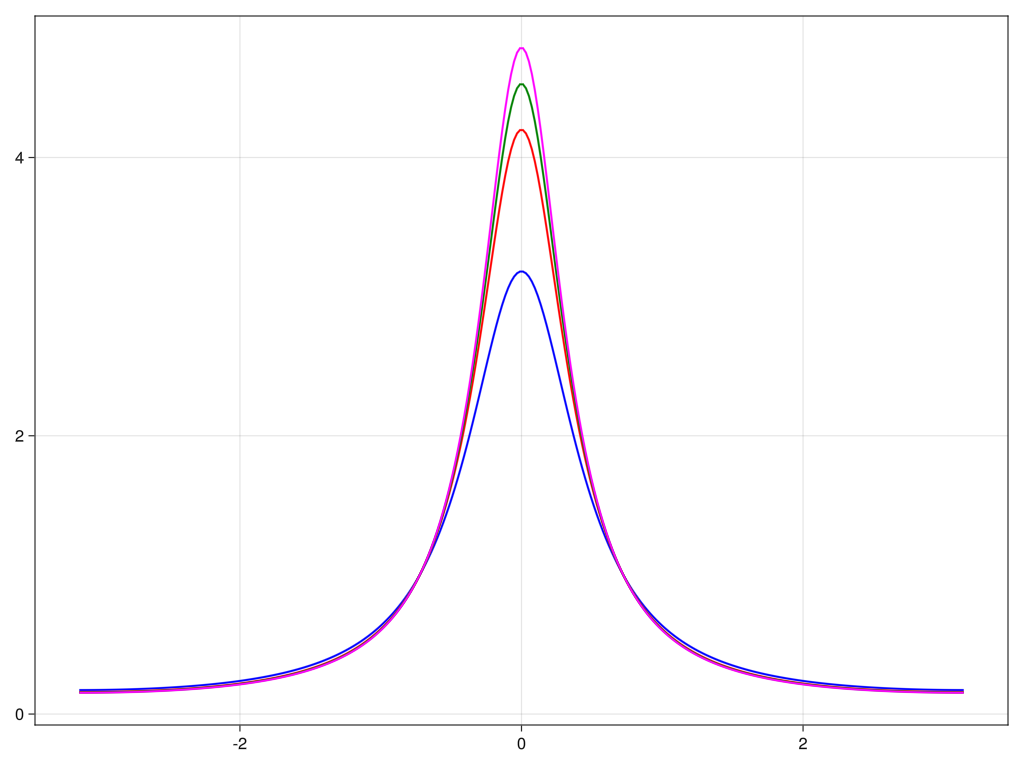
\includegraphics[width=0.50\textwidth]{CD_approx_example_1.png}} 
    \subfloat[]{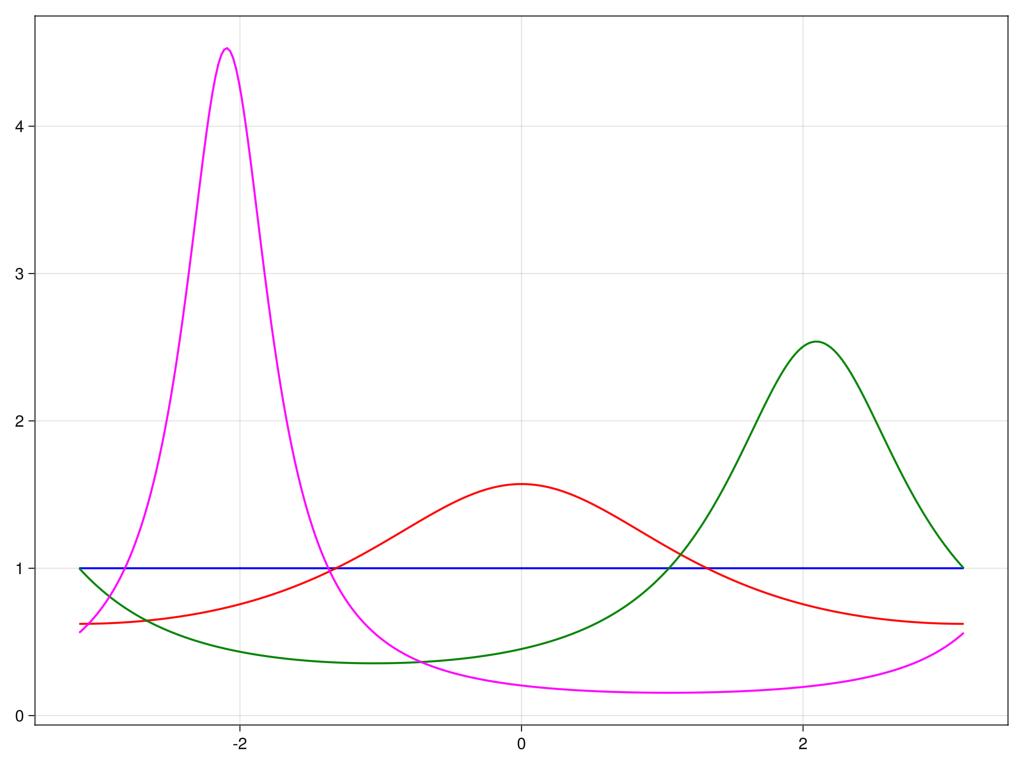
\includegraphics[width=0.50\textwidth]{CD_approx_example_2.png}} 
    \caption{(A) $(r_0,\theta_0)=(0.75,0.0)$ and degrees $2,4,5,6$ (B) $(r_0,\theta_0)$ in $(0,0)$, $(0.25,0)$, $(0.5,\pi/3)$ and $(0.75,4\pi/3)$ and degree $6$.}
    \label{fig: exit_loc_densities_SOS}
\end{figure}

\begin{figure}
    \centering
    \subfloat[]{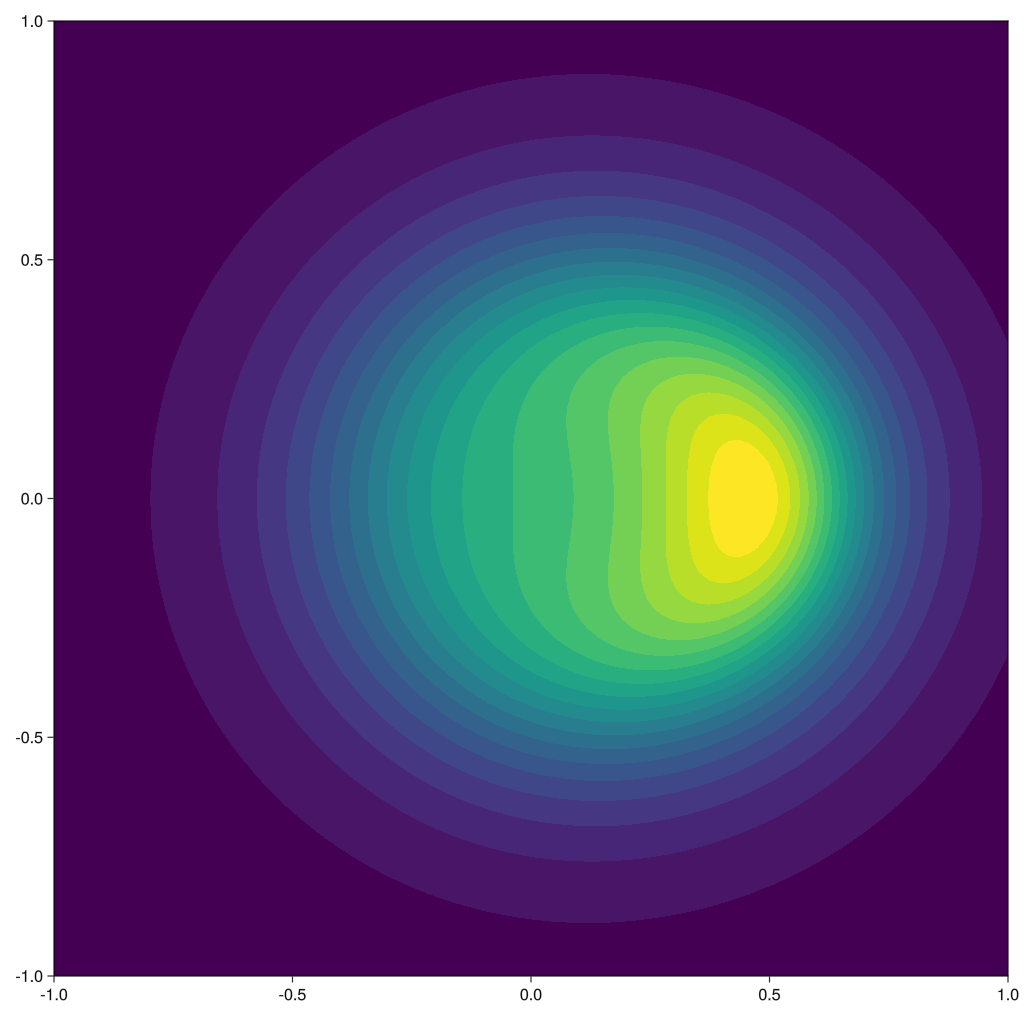
\includegraphics[width=0.30\textwidth]{CD_occupation_example_1b_dl2.png}} 
    \subfloat[]{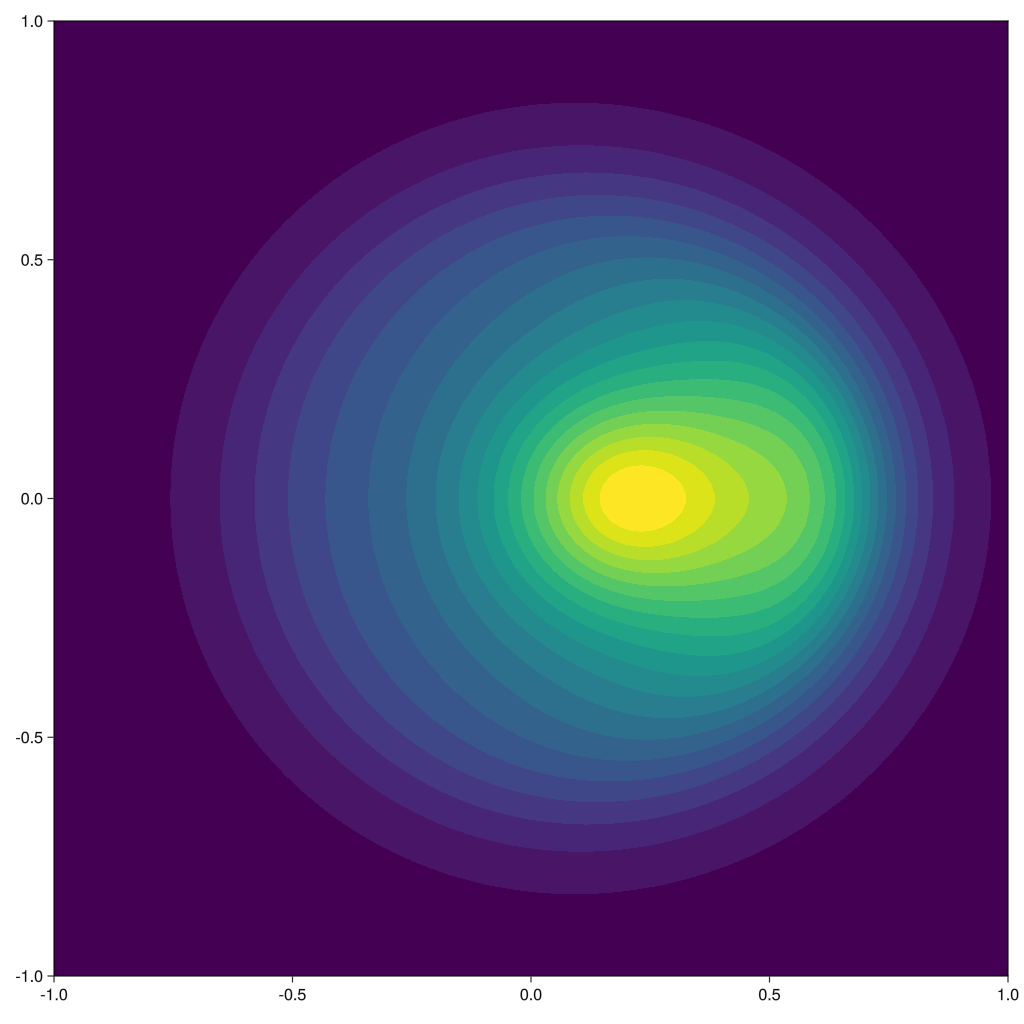
\includegraphics[width=0.30\textwidth]{CD_occupation_example_1b_dl3.png}} 
    \subfloat[]{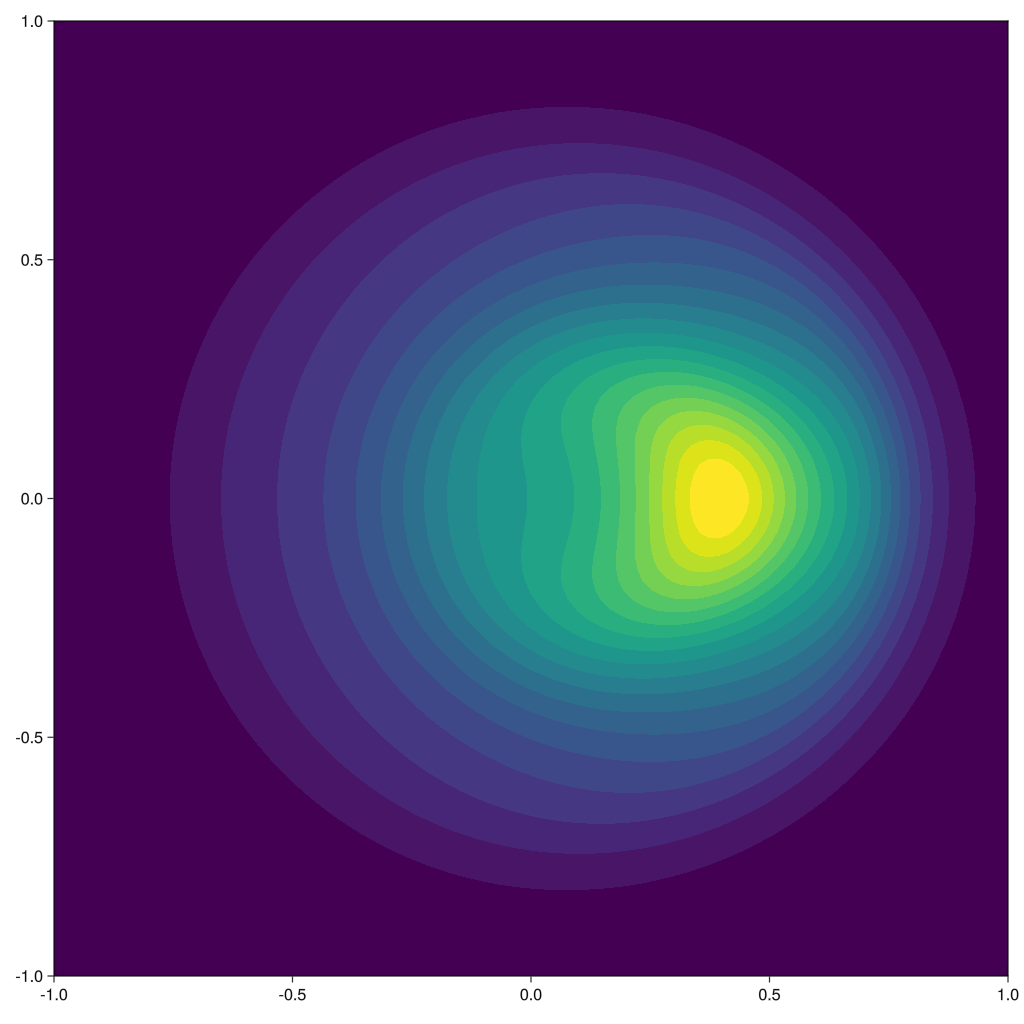
\includegraphics[width=0.30\textwidth]{CD_occupation_example_1b_dl4.png}} 
    \caption{Occupation density estimates in degrees Starting at $(r_0,\theta_0)=(0.25,0.0)$ using moment of degrees $2,4,7$}
    \label{fig: Brownian_Occupation}
\end{figure}


\end{examplex}

In our second example we study an instance of the so-called {\it polynomial diffusion models}. Such models play an imcreasingly important role in applications to finance as models of interest rates, credit risk and commodities and electricity~\cite{FilipovicLarsson}. Note that although the diffusion itself includes transcendental functions the corresponding infinitesimal operator maps polynomials to polynomials, allowing us to apply the techniques of the previous Section. This property explais the terminology ``polynomial'' in ``polynomial diffusion models''.


\begin{examplex} Consider a diffusion $(X_1,X_2)$ where $X_1$ is Brownian motion and $X_2$ is an independent squared Bessel process. More precisely, assume

\[
\left(\begin{array}{c}
dX_1(t)\\
dX_2(t)\\
\end{array}\right)
=
\left(\begin{array}{c}
0\\
\alpha\\
\end{array}\right)dt + 
\left(\begin{array}{cc}
1 & 0 \\
0 & 2\sqrt{X_2}
\end{array}\right)
\left(\begin{array}{c}
dW_1(t)\\
dW_2(t)\\
\end{array}\right)
\]
with $(X_1(0),X_2(0)) = (0.25,0)$. A simple calculation shows that
\[\mathcal{L}f=-\alpha \frac{\partial f}{\partial x_2}-\frac{1}{2}\frac{\partial^2 f}{\partial x_1^2}-2x_2\frac{\partial^2 f}{\partial x_2^2}.\] We apply the methodology from the previous Section to study the exit location and occupation densities. More specifically, Figure~\ref{fig: Bessel_loc_densities} shows the approximate exit location densities from the unit disc for various approximation degrees whereas Figure~\ref{fig: Bessel_Occup_densities} shows the occupation density for this process. 

\begin{figure}
    \centering
    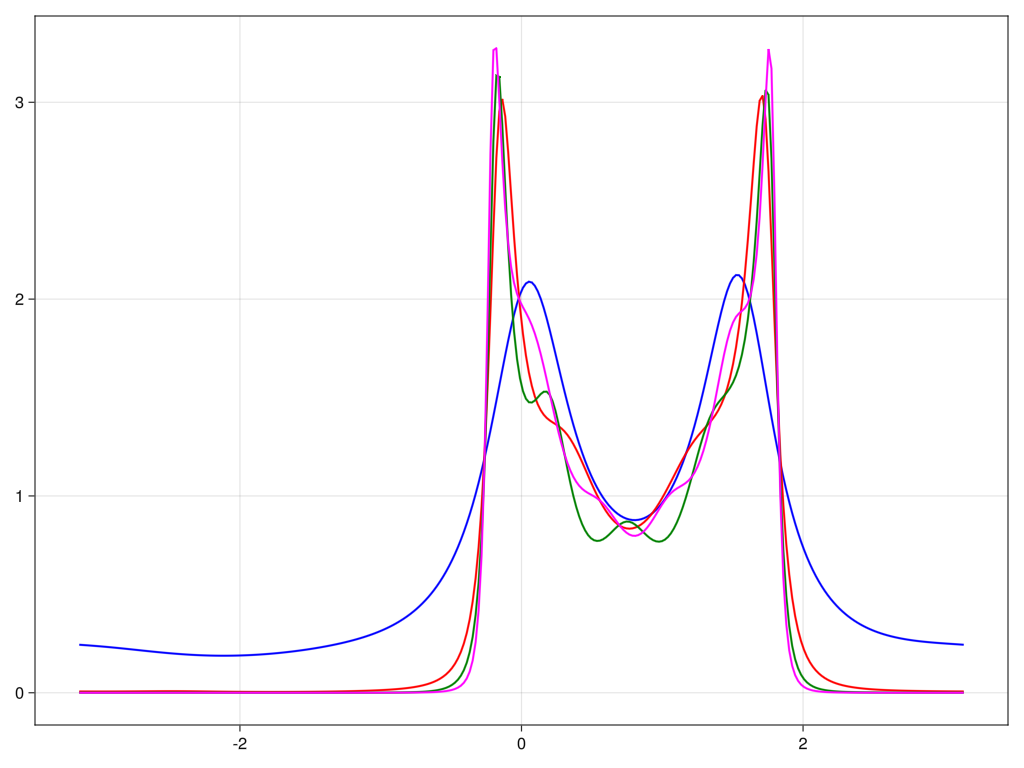
\includegraphics[width=0.70\textwidth]{CD_approx_example_3.png}
    \caption{Exit location density estimate from moments of degrees $2,4,6,7$ resp.}
    \label{fig: Bessel_loc_densities}
\end{figure}


\begin{figure}
    \centering
    \subfloat[]{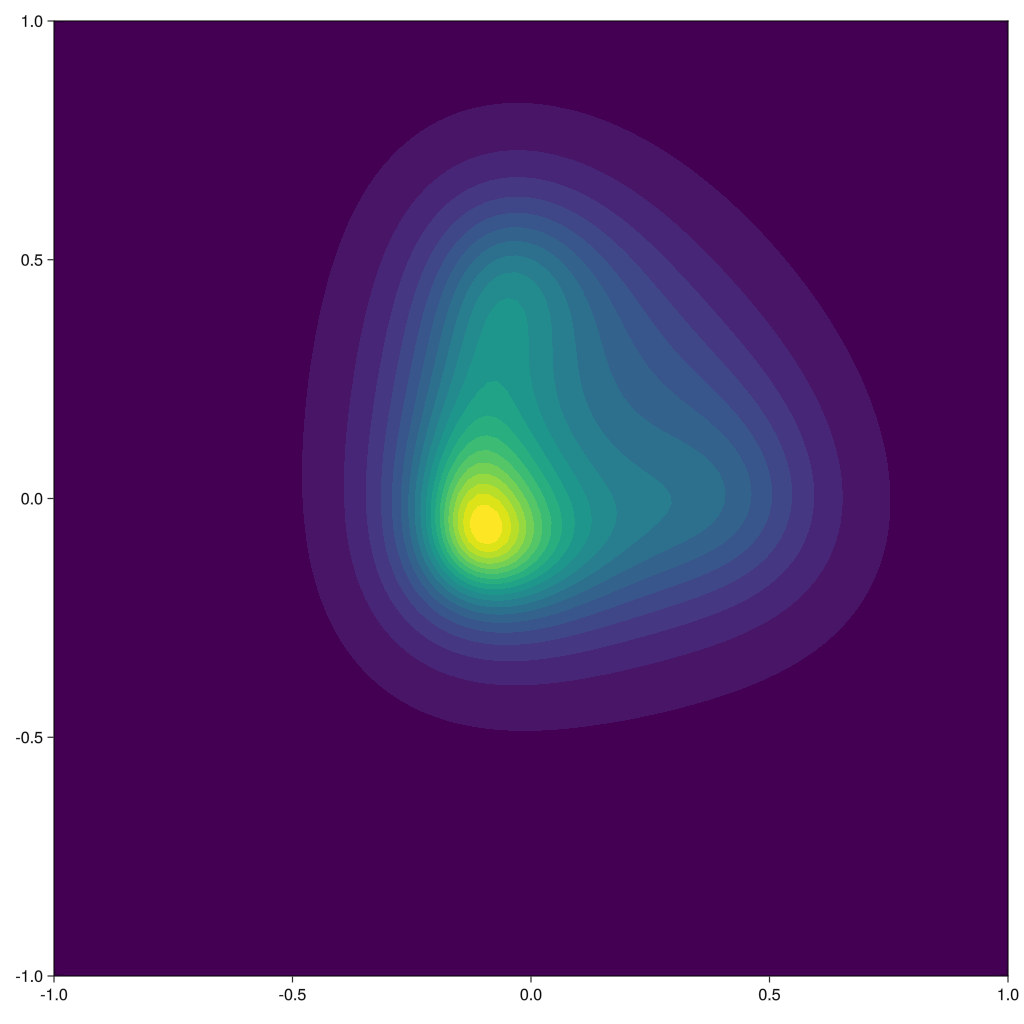
\includegraphics[width=0.50\textwidth]{CD_occupation_example_3b_dl2.png}} 
    \subfloat[]{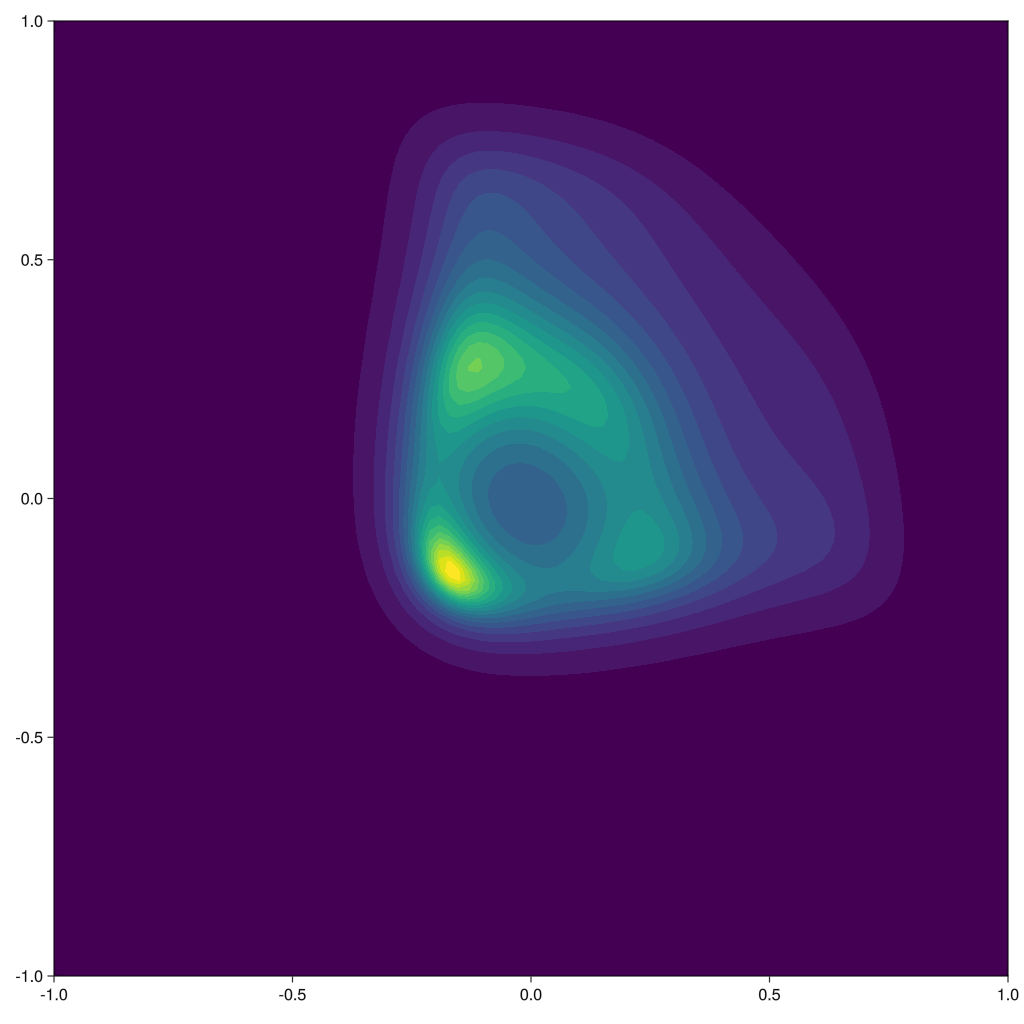
\includegraphics[width=0.50\textwidth]{CD_occupation_example_3b_dl3.png}} 
    \caption{Occupation density estimates from moments of degrees $2$ and $4$ resp.}
    \label{fig: Bessel_Occup_densities}
\end{figure}
\end{examplex}

\mv{It would be interesting to be able to obtain exit location densities from arbitrary semialgebraic sets (at least those that are closure of an open connected set), the difficulty being that one does not know the Equilibrium measure in general. I am thinking of developing a version of Lasserre's modified Kernel \url{https://arxiv.org/pdf/2301.11072.pdf}  "for boundaries" with an extra parameter $\epsilon$ and such that, suitably normalized, converges to the density as $\epsilon\rightarrow 0$. Interestingly this is exactly Young's mollifier idea we discussed long ago.}

\begin{bibdiv}
\begin{biblist}

\bib{LPPBook}{book}{
   author={Lasserre, Jean Bernard},
   author={Pauwels, Edouard},
   author={Putinar, Mihai},
   title={The Christoffel-Darboux kernel for data analysis},
   series={Cambridge Monographs on Applied and Computational Mathematics},
   volume={38},
   note={With a foreword by Francis Bach},
   publisher={Cambridge University Press, Cambridge},
   date={2022},
   pages={xv+168},
   isbn={978-1-108-83806-1},
   review={\MR{4394309}},
   doi={10.1017/9781108937078},
}
\bib{AzaisDeCastroGamboa}{article}{
   author={Aza\"\i s, Jean-Marc},
   author={de Castro, Yohann},
   author={Gamboa, Fabrice},
   title={Spike detection from inaccurate samplings},
   journal={Appl. Comput. Harmon. Anal.},
   volume={38},
   date={2015},
   number={2},
   pages={177--195},
   issn={1063-5203},
   review={\MR{3303671}},
   doi={10.1016/j.acha.2014.03.004},
}

\bib{KrooLubitsky2013a}{article}{
   author={Kro\'{o}, A.},
   author={Lubinsky, D. S.},
   title={Christoffel functions and universality in the bulk for
   multivariate orthogonal polynomials},
   journal={Canad. J. Math.},
   volume={65},
   date={2013},
   number={3},
   pages={600--620},
   issn={0008-414X},
   review={\MR{3043043}},
   doi={10.4153/CJM-2012-016-x},
}

\bib{FilipovicLarsson}{article}{
   author={Filipovi\'{c}, Damir},
   author={Larsson, Martin},
   title={Polynomial diffusions and applications in finance},
   journal={Finance Stoch.},
   volume={20},
   date={2016},
   number={4},
   pages={931--972},
   issn={0949-2984},
   review={\MR{3551857}},
   doi={10.1007/s00780-016-0304-4},
}
\end{biblist}

\end{bibdiv}


\end{document}

\subsection{Condition number estimates}

The method outlined in the previous sections allows us to estimate the moments of the exit location distribution or of the occupation measure on a collection of functions, together with error bounds on those estimates. It is natural to ask how do such errors affect the computed Christoffel function. More precisely we think of our Christoffel function computation as a map sending a matrix of moments $M$ to its corresponding function $\Lambda(M):=\frac{c}{\vec{m}^t M^{-1}\vec{m}}$ and we wish to estimate the condition number of $\Lambda$ where the norm on the space of symmetric matrices $\|M\|_{\infty}$ is the largest absolute value of any entry of $M$. Recall that the (relative) condition number of such a map is defined as
\[\hat{k}_{\Lambda}(M):= \lim_{\delta\rightarrow 0} \left\{\sup_{V: \|V\|_{\infty}\leq \delta} \left|\frac{\frac{\Lambda(M+V)-\Lambda(M)|}{\Lambda(M)}}{\|V\|_{\infty}/\|M\|_{\infty}}\right|\right\}\]
Our main result in this section is the following Theorem which gives an estimate of the relative condition number of $\Lambda$ in terms of the easily computable condition number of the moment matrix $M$, defined as the ratio $\frac{\sigma_1(M)}{\sigma_n(M)}$ 

\begin{theorem} Suppose $V$ is a vector space of continuous functions on $\partial \chi$ of dimension $N$ and suppose that the distribution of $\nu$ is supported on $\partial \chi$. If the moments of $M$ are known with componentwise error at most $\delta$ then the (relative) condition number of the Christoffel function satisfies the inequality
\[\hat{k}_\Lambda(M)\leq N \delta   \hat{k} (M)^2 = N \delta  \left(\frac{\sigma_1(M)}{\sigma_N(M)}\right)^2\]
\end{theorem}


\end{document}
